\documentclass[UTF8]{ctexart}

\usepackage{geometry}
\usepackage{listings}
\usepackage{natbib}
\usepackage{graphicx}
\usepackage{subcaption}
\usepackage{algorithm}
\usepackage{amsmath}
\usepackage[noend]{algpseudocode}
\usepackage{lmodern}
\usepackage{url}
\usepackage{verbatim}
\usepackage{multirow}
\usepackage{hhline}

\lstset{frame=tb,
  aboveskip=3mm,
  belowskip=3mm,
  showstringspaces=false,
  columns=flexible,
  basicstyle={\small\ttfamily},
  numbers=none,
  numberstyle=\tiny\color{gray},
  breaklines=true,
  breakatwhitespace=true,
  tabsize=3
}

\geometry{left=4cm,right=4cm,top=3cm,bottom=3cm}

\title{单链表回路问题的三种算法的性能比较与分析}
\author{何昊}

\begin{document}

\maketitle

\section{引言}

链表是程序设计中最基本的数据结构之一。对于一个维护线性地址空间的程序而言,这个程序中的某个数据结构要么利用一段连续的内存,要么利用多段不连续的内存来保存其所需要的数据。对于后者而言,最简单的数据结构就是链表。链表虽然简单,但是在实际的算法和系统中有广泛的应用。例如,邻接链表可以用于表示一个图和解决哈希表的碰撞问题\cite{cormen2009introduction};链表可以用来实现动态内存管理\cite{bryant2003computer};等等。

对于以上使用链表的程序而言,保证链表的正确性很重要,其中尤其重要的是链表不能有环。在链表上运行的哪怕是最基本的算法,都会因为链表存在环而出现问题。例如,任何一个遍历链表的算法都会因为环而陷入死循环。因此,在程序运行时对链表进行高效的环路检查,对于测试软件正确性非常重要\cite{auguston1997assertions}。此外,链表回路的检测算法也可应用于伪随机数生成器分析\cite{knuth2014art}、密码学\cite{quisquater1989easy}、程序分析\cite{van1987efficient}、力学模拟\cite{fich1981lower}等等领域。

以上问题被称作\textbf{单链表回路问题}。已经存在多种高效算法可以用来解决单链表回路问题,其中比较著名的有\textbf{赛跑法}、\textbf{翻转法}和\textbf{指向自身法}三种。对这三种算法的性能的细致比较,将会有助于在实际应用场景中选择最合适的算法。因此,在本文中,我们对这三种算法的时间和空间性能,进行理论和实验上的比较与分析。我们发现,对于长度为$m+n$,环的长度为$n$的链表,三种算法的时间复杂度均为$O(m+n)$;赛跑法和翻转法的空间复杂度为$O(1)$,而指向自身法的空间复杂度为$O(m+n)$。在实验中,我们发现,在要求保留原链表结构和不允许内存泄露的前提下,赛跑法拥有最优秀的运行时间和运行时内存消耗;翻转法的内存消耗与赛跑法接近而运行时间略慢;指向自身法在运行时间上和内存消耗上都差于前两者。因此,本文建议在实际应用中,使用赛跑法来解决单链表回路问题。

本文的余下部分是这样组织的。第二节将会详细介绍三种解决单链表回路问题的算法;第三节将会对三种算法的理论性能,包括时间复杂度和空间复杂度进行分析;第四节将会从实验的角度评测这三种算法的实际时间和空间性能;最后,在第五节得出结论。

\section{解决方案介绍}

\subsection{赛跑法}

赛跑法的基本思想是,在遍历链表的过程中,使用一个快指针和慢指针从头开始遍历。在每次遍历时,快指针前进两个节点,慢指针前进一个节点。如果快指针到达链表结尾,则链表没有环。如果在某次迭代中快指针与慢指针指向同一个节点,则链表中有环。赛跑法不仅不需要额外内存空间,也不用对链表进行任何写操作。赛跑法的C++实现如下。

\begin{lstlisting}
struct Node {
    Node *next;
};
bool has_cycle_running(Node *lst) {
    Node *fast = lst;
    Node *slow = lst;
    while (true) {
        fast = fast->next;
        if (fast == nullptr) return false;
        if (fast == slow) return true;
        fast = fast->next;
        if (fast == nullptr) return false;
        if (fast == slow) return true;
        slow = slow->next;
        if (fast == slow) return true;
    }
}
\end{lstlisting}

\subsection{翻转法}

翻转法的基本思想是,在遍历链表的过程中,每次使用两个指针将链表的节点进行翻转,让子节点指向父节点。如果一直翻转到最后又回到了头部节点,则链表存在环。如果翻转到最后遇到一个没有子节点的节点,则链表不存在环。翻转法也不需要额外内存空间,且可以在运行完之后将链表恢复成原来的状态。翻转法的C++实现如下。

\begin{lstlisting}
bool reverse(Node *lst, Node **tail) {
    Node *prev = nullptr;
    Node *curr = lst;
    while (curr != nullptr) {
        Node *temp = curr->next;
        curr->next = prev;
        *tail = prev = curr;
        curr = temp;
        if (curr == lst) {
            curr->next = prev;
            return true;
        }
    }
    return false;
}

bool has_cycle_reverse(Node *lst) {
    Node *tail = nullptr;
    bool result = reverse(lst, &tail);
    if (result) reverse(lst, &tail);
    else reverse(tail, &tail);
    return result;
}
\end{lstlisting}

\subsection{指向自身法}

指向自身法的核心思想是,在遍历链表的过程中,将每个节点指向自身。如果在遍历途中遇到一个已经指向自身的节点,则链表存在环。如果没有遇到这样的节点而达到了链表结尾,则链表不存在环。这个算法运行完后,必须借助额外数据结构,才能将链表恢复成原来的状态,或者对链表节点进行垃圾回收。指向自身法的C++实现如下。

\begin{lstlisting}
bool has_cycle_pointself(Node* lst) {
    bool result = false;
    Node *curr = lst;
    std::vector<Node *> visited;
    while (curr != nullptr) {
        if (curr->next == curr) {
            result = true;
            break;
        }
        visited.push_back(curr);
        Node *temp = curr->next;
        curr->next = curr;
        curr = temp;
    }
    for (Node *n : visited) delete n;
    return result;
}
\end{lstlisting}

\section{理论性能分析}

在本节中,我们利用大$O$表示法对三种算法的时间复杂度和空间复杂度进行分析。在单链表回路问题中,输入数据中任何一个链表都可以用唯一的整数二元组$\langle m, n \rangle$表示,其中$m$为链表中不是环的部分的长度,$n$为环的长度。对于没有环的链表而言,$n=0$。

对于赛跑法而言,我们分以下两种情况讨论。对于没有环的链表($n=0$),当快指针达到链表末尾时停止,时间复杂度为$O(m)$;对于有环的链表,当慢指针走过$m$个节点进入环时,快指针已经在环里,此时快指针最多走过$n$个节点就能追上慢指针,因此慢指针最多走过$m+n/2$个节点后算法停止,时间复杂度为$O(m+n)$。赛跑法需要的额外的空间只有两个指针和若干临时变量,因此空间复杂度为$O(1)$。

对于翻转法而言,我们也分成两种情况讨论。对于没有环的链表($n=0$),算法在走到链表末尾时停止,时间复杂度为$O(m)$;对于有环的链表,算法会回到链表开头时停止,遍历$2m+n$个节点,时间复杂度为$O(m+n)$。翻转法需要的额外空间也只有两个指针和若干临时变量,因此空间复杂度为$O(1)$。

对于指向自身法而言,对于没有环的链表和有环的链表,算法都会在遍历$m+n$个节点后停止,因此时间复杂度为$O(m+n)$。然而,如果需要恢复链表或对链表进行存储空间回收,算法在运行过程中必须保存遍历过的节点,因此空间复杂度为$O(m+n)$。

三种算法的时间复杂度和空间复杂度总结见表\ref{tab:complexity}。

\begin{table}
\centering
\begin{tabular}{lll}
 算法 & 时间复杂度 & 空间复杂度 \\ 
\hhline{===}
赛跑法 & $O(m+n)$ & $O(1)$  \\ 
\hline
翻转法 & $O(m+n)$ & $O(1)$  \\ 
\hline
指向自身法 & $O(m+n)$ & $O(m+n)$
\end{tabular}
\caption{三种单链表回路算法的时间复杂度与空间复杂度}
\label{tab:complexity}
\end{table}

\section{实际性能评测}

\subsection{实验设计}

对于理论复杂度相同的算法,我们也需要知道他们在实际中性能区别。因此在本节中,我们将会通过试验对对三种解决单链表回路问题的算法的时间性能和空间性能进行评测。我们首先构建评测数据集。我们希望评测集中包含不同长度数量级的链表,并且对每种链表长度,其中的环的大小不同。正如前文所说,整数二元组$\langle m, n\rangle$可以唯一表示一个链表,因此我们构建$m, n$满足如下条件的链表集合作为我们评测集

$$
m+n\in \{10^6, 2 \times 10^6, 4 \times 10^6, 6 \times 10^6, 8 \times 10^6, 10^7, 2\times 10^7, 3\times 10^7, 4\times 10^7, 5\times 10^7\}
$$
$$
n = x(m + n), x \in \{0, 0.1, 0.2, 0.3, ..., 0.9, 1.0\}
$$

其中,$m+n$的最大取值受限于评测机器的内存大小。然后,对于每种算法,我们通过可视化分析,比较其在不同输入数据下的运行时间和运行过程中最大的内存消耗,从而得到三种算法性能特征的实验性结果。


\subsection{实现细节}

我们的实验机器是MacBook Pro 2016, 2.1GHz CPU, 8GB RAM,操作系统是Mac OS X。为了尽可能避免语言运行时开销对算法性能分析带来的影响,我们选用C++语言来实现上述三种单链表回路算法。在实现中,为了尽可能贴近真实场景的链表使用情况,我们规定

\begin{itemize}
\item 算法在结束时,原链表的结构必须保持原状
\item 算法不应当产生内存泄漏
\end{itemize}

我们在评测机器上使用Shell脚本提供的\texttt{time}命令统计运行时间和运行过程的最大内存消耗,并输出成CSV表格供后续分析。为了避免运行过程中的随机误差,我们对每个链表,每种算法运行20次取内存消耗和时间消耗的平均值。然后,我们使用Python对不同算法在不同输入数据下的时间和空间消耗情况进行可视化分析。实验使用的代码、数据和分析参见\footnote{\url{https://github.com/hehao98/CycleInLinkedList}}。

\subsection{实验结果}

\begin{figure}[h]
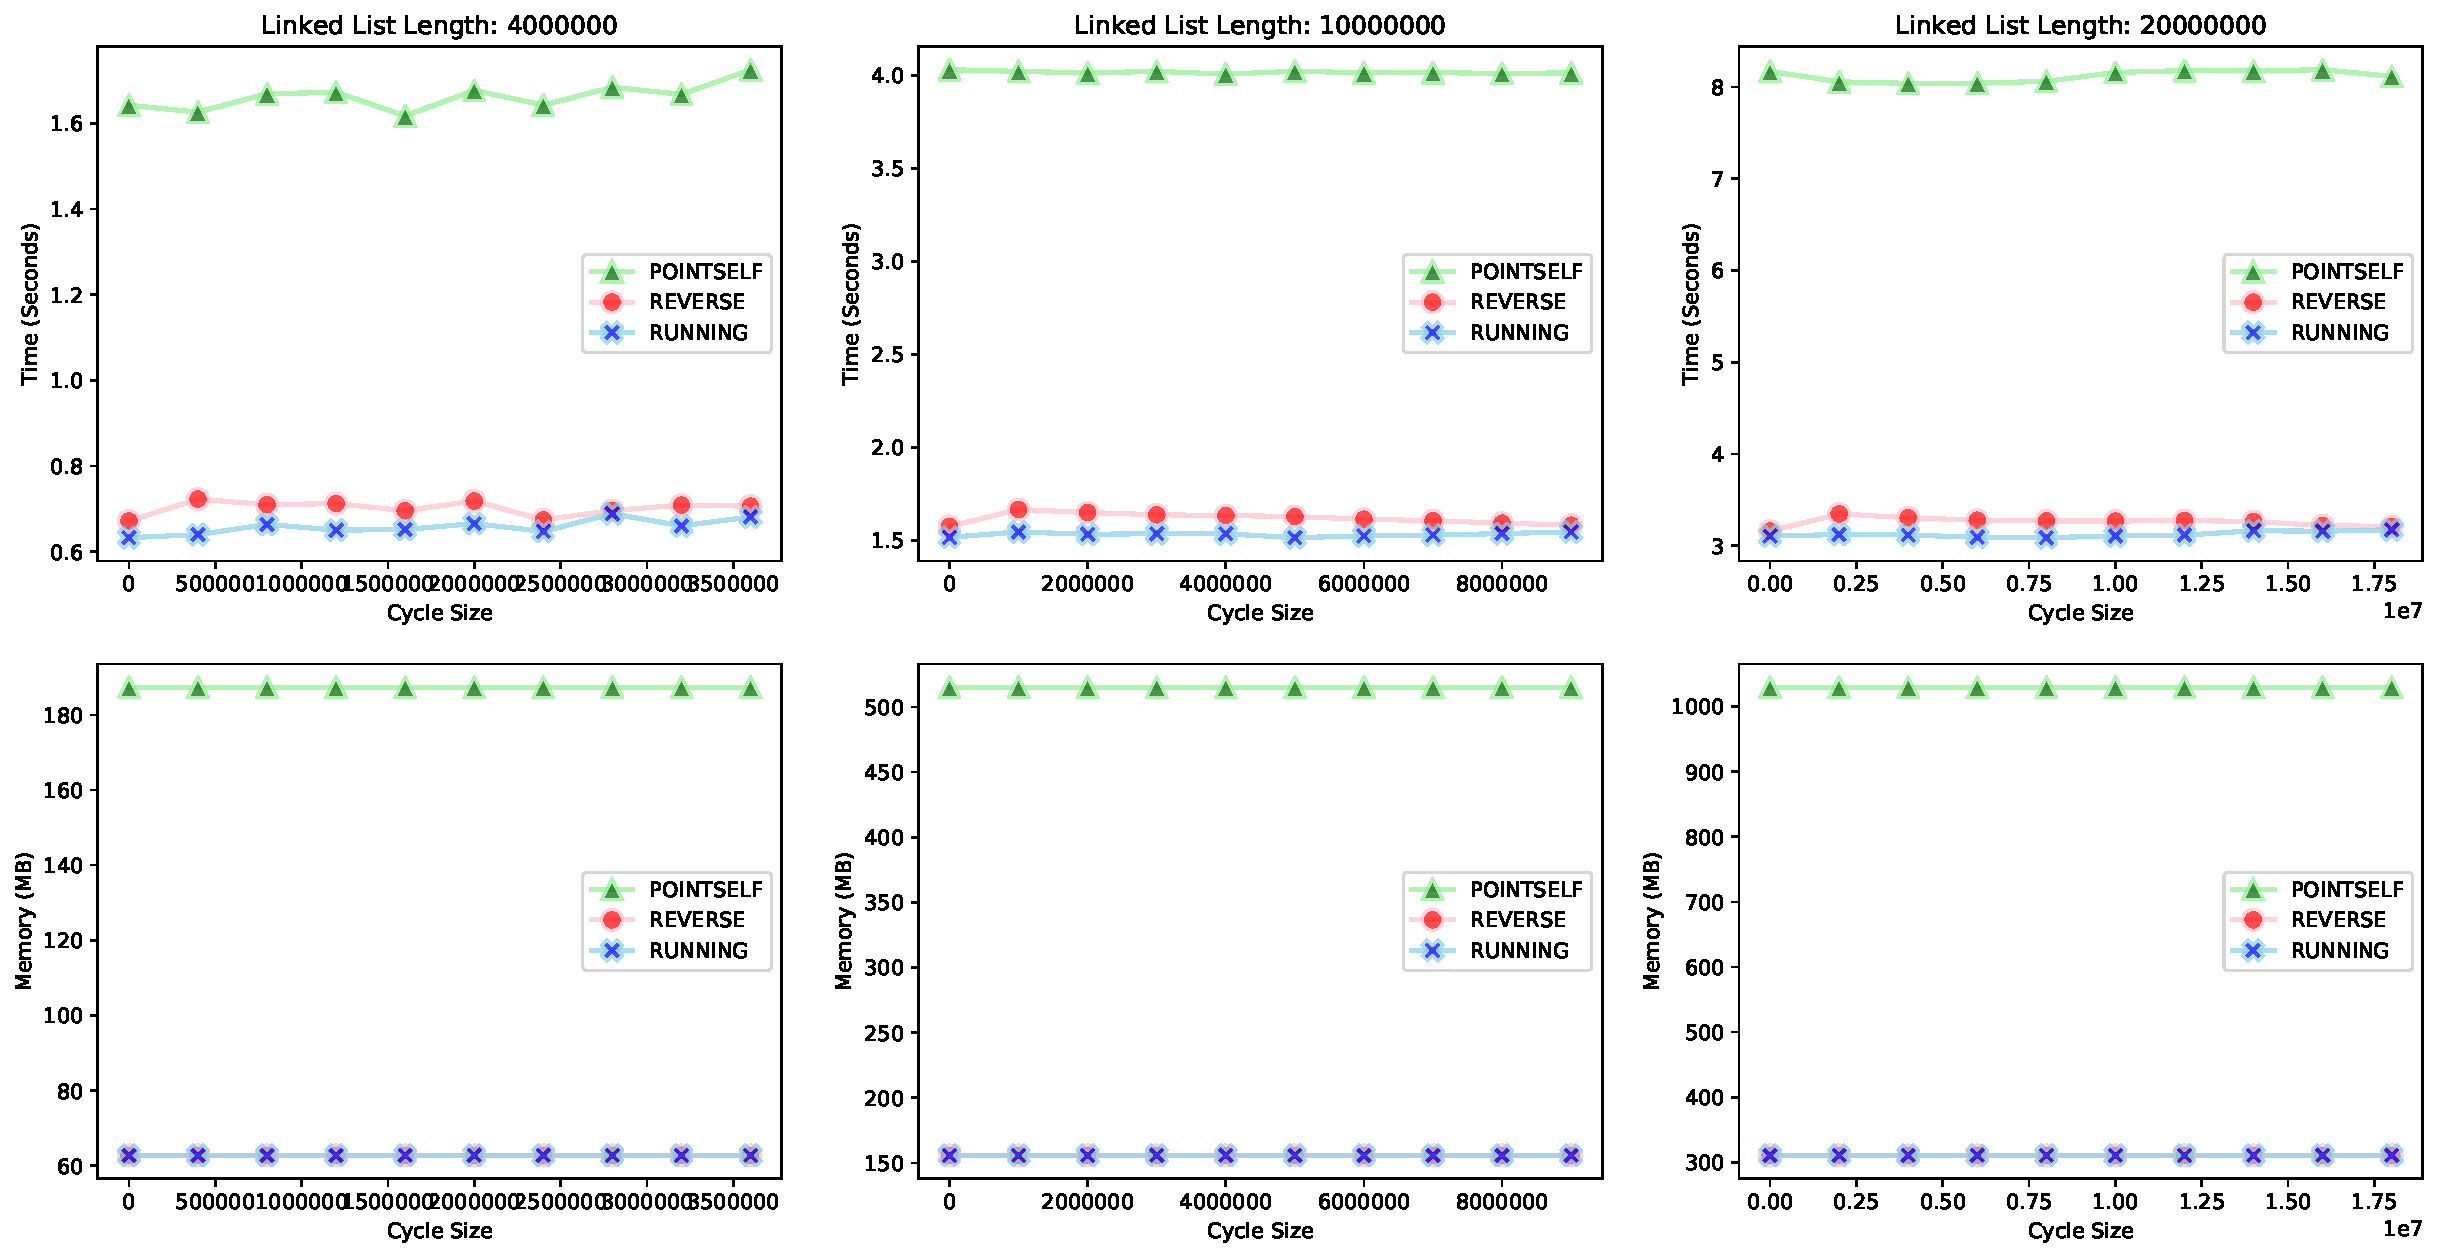
\includegraphics[width=\textwidth]{fig.pdf}
\caption{三种算法在不同链表长度下的时间与空间消耗。横坐标是环的大小}
\label{fig1}
\end{figure}

\begin{figure}
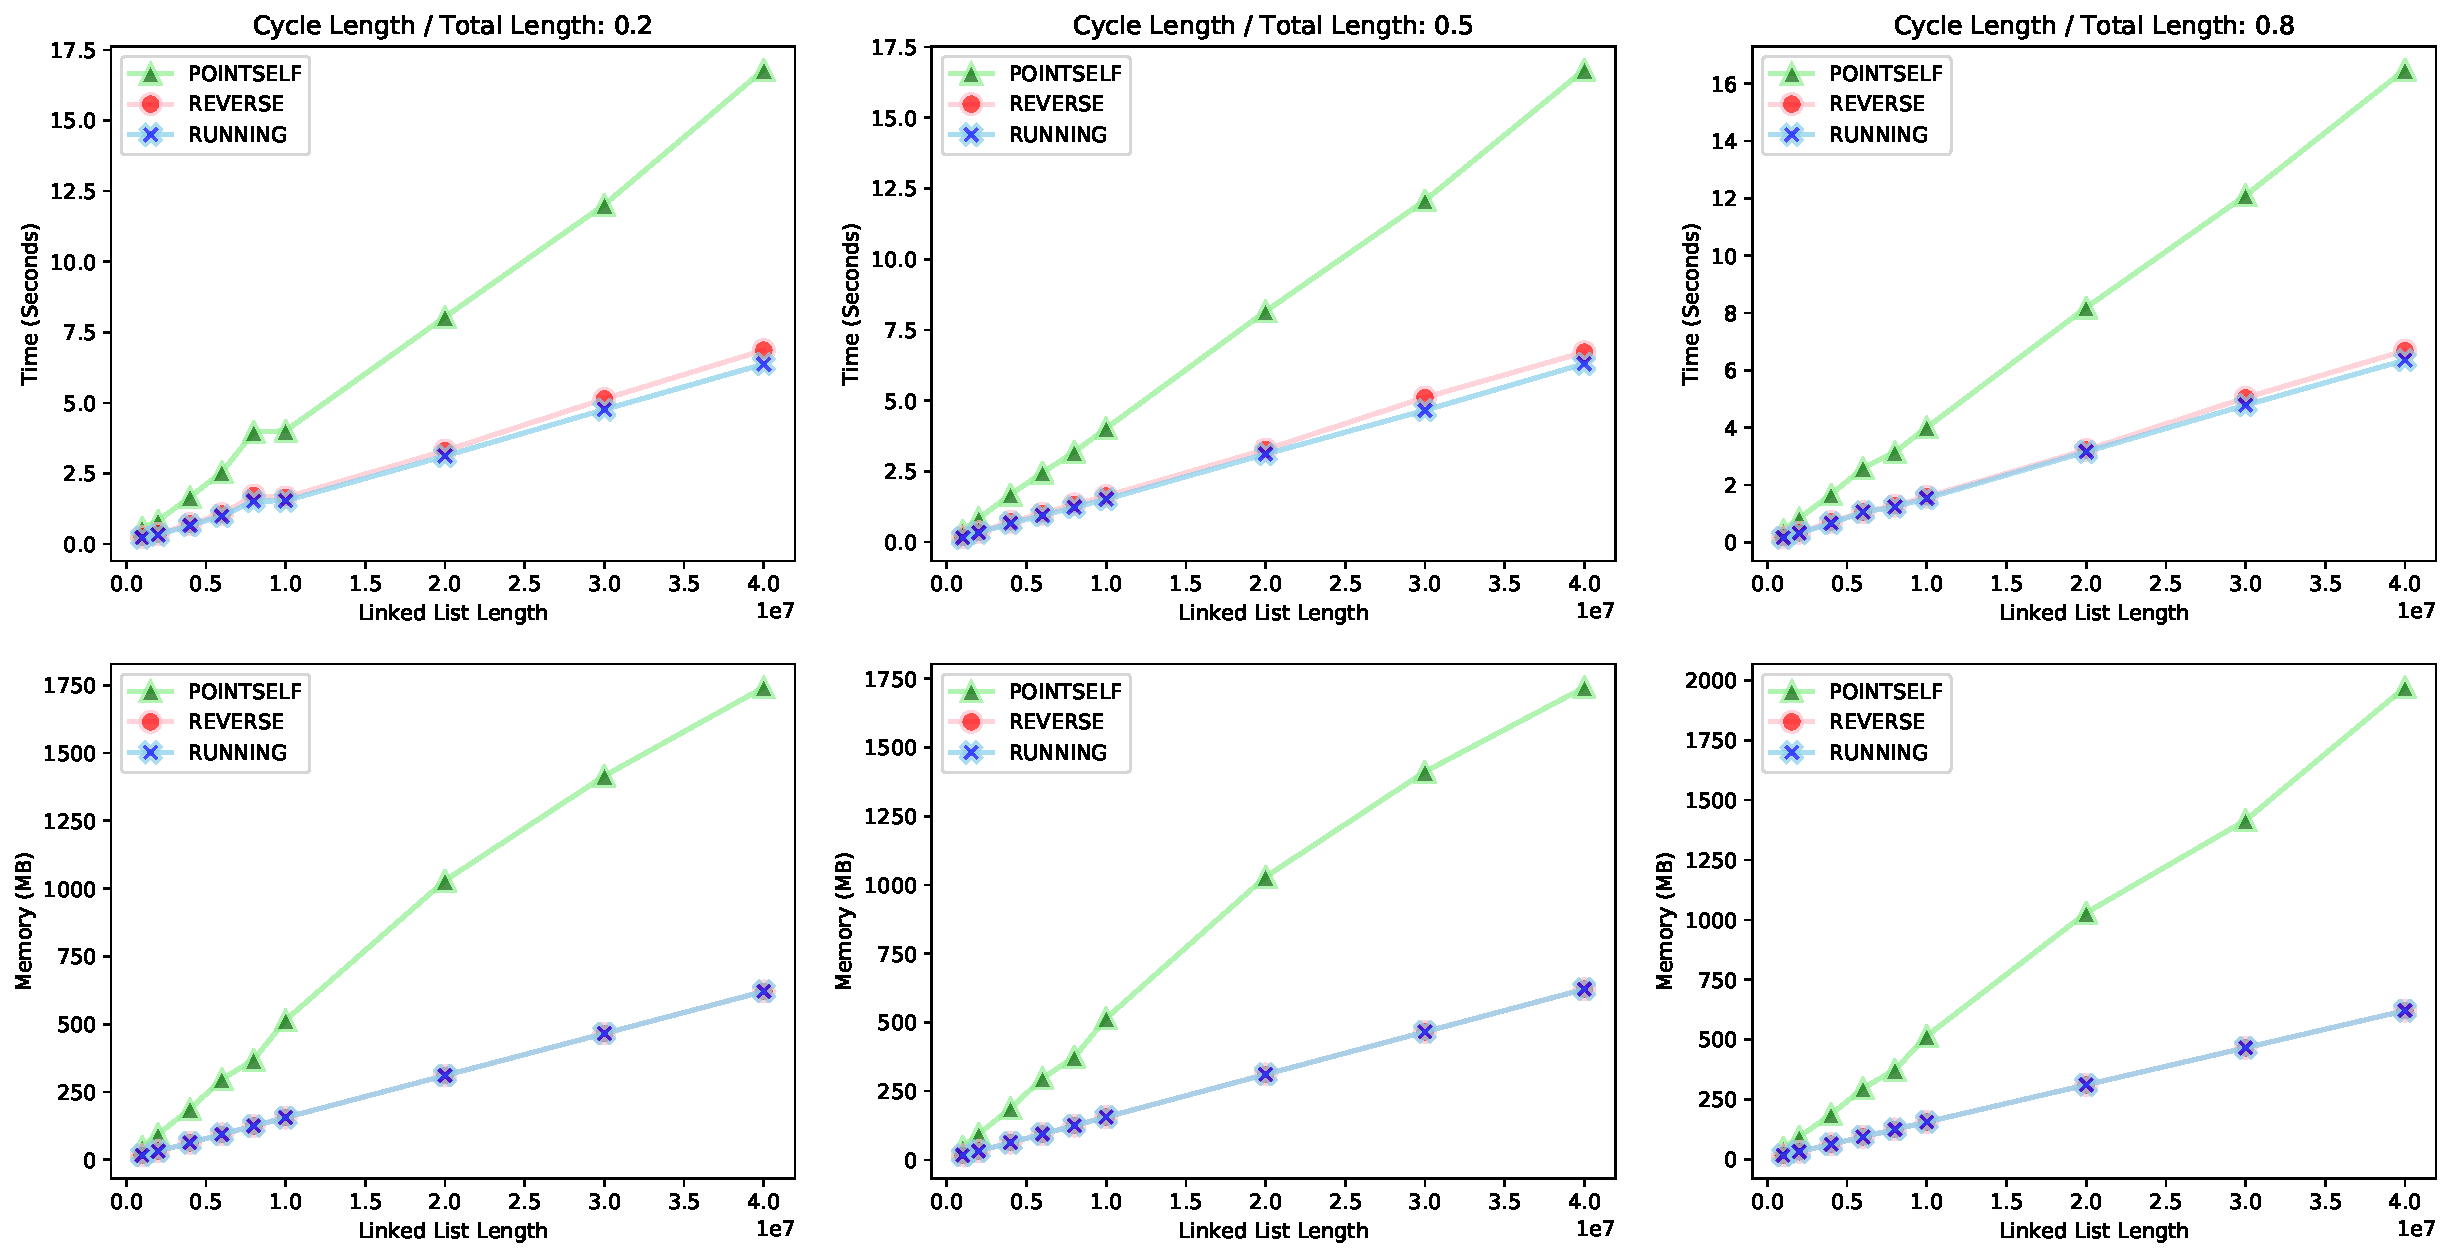
\includegraphics[width=\textwidth]{fig2.pdf}
\caption{三种算法的时间与空间消耗随着总链表长度的变化}
\label{fig2}
\end{figure}

图\ref{fig1}和图\ref{fig2}以不同的形式展示了三种算法在评测数据集上的时间和空间性能。图中,\texttt{RUNNING}表示赛跑法;\texttt{REVERSE}表示翻转法;\texttt{POINTSELF}表示指向自身法。在图\ref{fig1}中,我们可以看到,在总长度$m+n$一定的情况下,环$n$的大小对三种算法的时间和空间性能都没有决定性影响,这与之前理论复杂度分析的结果是一致的。然而,由于指向自身法会消耗更多的额外空间,因此运行时不仅内存开销更大,连运行时间都比赛跑法和指向自身法更慢。然后,实验中赛跑法的运行时间快于翻转法,这可能是因为翻转法在运行后必须消耗额外的计算开销将链表恢复成原来的状态。在图\ref{fig2}中,我们可以看到,不管环有多大,算法的时间消耗和空间消耗都是随着链表长度线性增长的关系,这与之前的理论分析的结果是一致的(尽管赛跑法和翻转法的额外空间消耗是$O(1)$,但是链表本身需要$O(n)$的空间)。此外,我们可以看到,翻转法和赛跑法在空间开销上几乎是一样的,而赛跑法略快于翻转法。

\section{结论}

通过实验和理论分析,我们发现,在要求不产生内存泄漏和必须保持原链表结构的情况下,指向自身法不仅内存开销大,运行时间也更慢;赛跑法和反转法都不产生额外的内存开销,且赛跑法比反转法要快;而且对于只读的链表而言,只能运行赛跑法。因此,实际实践中,应该使用赛跑法来解决单链表环路问题。


\bibliographystyle{plain}
\bibliography{references}
\end{document}